\documentclass[12pt]{article}
\usepackage[a4paper, margin=1in]{geometry}
\usepackage{graphicx}
\usepackage{setspace}
\usepackage{titlesec}
\usepackage{amsmath, amssymb}
\usepackage{hyperref}
\setstretch{1.15}
\titleformat{\section}{\large\bfseries}{\thesection.}{0.5em}{}

\begin{document}
	
	\begin{center}
		{\LARGE \textbf{Donor and Acceptor Levels in Semiconductors}}\\[0.5em]
		{\large Summary Note for Semiconductor Physics}
	\end{center}
	\vspace{1em}
	
	\section{Intrinsic Semiconductor Baseline}
	In a pure (intrinsic) semiconductor such as silicon:
	\begin{itemize}
		\item The valence band is completely filled with electrons.
		\item The conduction band is empty at \(0\,\text{K}\).
		\item The bandgap \(E_g = E_c - E_v \approx 1.1\,\text{eV}\).
	\end{itemize}
	Electrons must be thermally excited across this gap to contribute to conduction, which is inefficient at low temperature. Doping introduces shallow energy levels to make this process easier.
	
	\section{Donor Levels (n-Type Doping)}
	When a donor atom such as phosphorus is introduced into silicon:
	\begin{itemize}
		\item Phosphorus has five valence electrons; four form covalent bonds, leaving one extra electron.
		\item This extra electron is weakly bound to the donor atom, creating a discrete energy level slightly below the conduction band edge \(E_c\).
		\item This state, called the \textbf{donor level} \(E_d\), is where the donor electron \textbf{sits before ionization}.
		\item The \textbf{donor ionization energy} is the small energy needed to free that electron into the conduction band:
		\[
		E_c - E_d \approx 50\,\text{meV}.
		\]
	\end{itemize}
	At room temperature, \(kT \approx 25\,\text{meV}\), so most donor electrons are thermally ionized, producing free conduction electrons and resulting in \textbf{n-type conductivity}.
	
	\section{Acceptor Levels (p-Type Doping)}
	When an acceptor atom such as boron is introduced:
	\begin{itemize}
		\item Boron has only three valence electrons and can accept one electron from a neighboring Si bond.
		\item This creates a \textbf{hole} in the valence band and an \textbf{acceptor level} \(E_a\) just above the valence band edge \(E_v\).
		\item The \textbf{acceptor level} represents the energy state the captured electron occupies \textbf{before ionization}, i.e., before the hole is freed into the valence band.
		\item The \textbf{acceptor ionization energy} is the energy required to excite a valence electron into the acceptor level:
		\[
		E_a - E_v \approx 50\,\text{meV}.
		\]
	\end{itemize}
	This process generates holes in the valence band, giving the material \textbf{p-type conductivity}.
	
	\section{Energy-Level Diagram}
	Figure~\ref{fig:donor_acceptor} illustrates these energy levels schematically.
	
	\begin{figure}[h!]
		\centering
		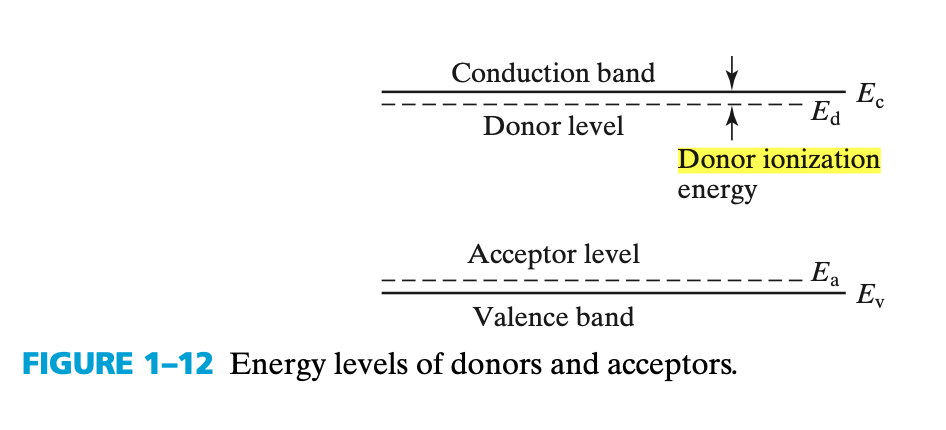
\includegraphics[width=0.75\linewidth]{donor_acceptor_level.png}
		\caption{Energy levels of donors and acceptors (adapted from Chenming Hu). 
			The donor electron initially occupies the donor level \(E_d\), located just below the conduction band edge \(E_c\). 
			Ionizing the donor requires an energy \(E_c - E_d\) (the donor ionization energy) to lift this electron into the conduction band. 
			Similarly, an acceptor level \(E_a\) lies just above the valence band \(E_v\); before ionization, it can capture an electron from the valence band, leaving behind a mobile hole.}
		\label{fig:donor_acceptor}
	\end{figure}
	
	\section{Summary}
	\begin{itemize}
		\item \textbf{Donor level:} Shallow energy level introduced by a donor atom, typically \(E_d \approx 50\,\text{meV}\) below \(E_c\). The donor electron resides here \emph{before ionization}.
		\item \textbf{Acceptor level:} Shallow energy level introduced by an acceptor atom, typically \(E_a \approx 50\,\text{meV}\) above \(E_v\). It represents the bound state of the captured electron before the hole is freed.
		\item These shallow levels drastically increase carrier concentration without significantly disturbing the band structure.
	\end{itemize}
	
	\noindent
	\textbf{In one sentence:} 
	Dopant atoms create shallow electronic states within the bandgap---just below \(E_c\) for donors or just above \(E_v\) for acceptors---and the small ionization energy ($\sim50$\,meV) is sufficient to free carriers into the conduction or valence bands.
	
\end{document}
